\documentclass[12pt,a4]{article}
\usepackage[]{graphicx}\usepackage[]{xcolor}
% maxwidth is the original width if it is less than linewidth
% otherwise use linewidth (to make sure the graphics do not exceed the margin)
\makeatletter
\def\maxwidth{ %
  \ifdim\Gin@nat@width>\linewidth
    \linewidth
  \else
    \Gin@nat@width
  \fi
}
\makeatother

\definecolor{fgcolor}{rgb}{0.345, 0.345, 0.345}
\newcommand{\hlnum}[1]{\textcolor[rgb]{0.686,0.059,0.569}{#1}}%
\newcommand{\hlstr}[1]{\textcolor[rgb]{0.192,0.494,0.8}{#1}}%
\newcommand{\hlcom}[1]{\textcolor[rgb]{0.678,0.584,0.686}{\textit{#1}}}%
\newcommand{\hlopt}[1]{\textcolor[rgb]{0,0,0}{#1}}%
\newcommand{\hlstd}[1]{\textcolor[rgb]{0.345,0.345,0.345}{#1}}%
\newcommand{\hlkwa}[1]{\textcolor[rgb]{0.161,0.373,0.58}{\textbf{#1}}}%
\newcommand{\hlkwb}[1]{\textcolor[rgb]{0.69,0.353,0.396}{#1}}%
\newcommand{\hlkwc}[1]{\textcolor[rgb]{0.333,0.667,0.333}{#1}}%
\newcommand{\hlkwd}[1]{\textcolor[rgb]{0.737,0.353,0.396}{\textbf{#1}}}%
\let\hlipl\hlkwb

\usepackage{framed}
\makeatletter
\newenvironment{kframe}{%
 \def\at@end@of@kframe{}%
 \ifinner\ifhmode%
  \def\at@end@of@kframe{\end{minipage}}%
  \begin{minipage}{\columnwidth}%
 \fi\fi%
 \def\FrameCommand##1{\hskip\@totalleftmargin \hskip-\fboxsep
 \colorbox{shadecolor}{##1}\hskip-\fboxsep
     % There is no \\@totalrightmargin, so:
     \hskip-\linewidth \hskip-\@totalleftmargin \hskip\columnwidth}%
 \MakeFramed {\advance\hsize-\width
   \@totalleftmargin\z@ \linewidth\hsize
   \@setminipage}}%
 {\par\unskip\endMakeFramed%
 \at@end@of@kframe}
\makeatother

\definecolor{shadecolor}{rgb}{.97, .97, .97}
\definecolor{messagecolor}{rgb}{0, 0, 0}
\definecolor{warningcolor}{rgb}{1, 0, 1}
\definecolor{errorcolor}{rgb}{1, 0, 0}
\newenvironment{knitrout}{}{} % an empty environment to be redefined in TeX

\usepackage{alltt}
\newcommand{\SweaveOpts}[1]{}  % do not interfere with LaTeX
\newcommand{\SweaveInput}[1]{} % because they are not real TeX commands
\newcommand{\Sexpr}[1]{}       % will only be parsed by R



% ---- Metadata ---- %

\title{Honesty by Convenience: Corruption Tolerance in Ecuador}
\author{Daniel Hernán Sánchez Pazmiño}
\date{June 2022}

% ---- Load Packages ---- %

% Math

\usepackage{savesym} % Need to "save" the command that is already defined \varTheta

\usepackage{amsmath}
  \savesymbol{varTheta} 

% Fonts

% To set the TNR font for both text and equations:

\usepackage{mathspec}
  \setallmainfonts(Digits,Greek,Latin){Times New Roman}
\restoresymbol{MTP}{varTheta}

% Formatting

\usepackage{setspace}
  \doublespacing

\usepackage[margin = 1in]{geometry}

\usepackage{lscape}

% Citation & Bibliographies

\usepackage[backend = biber, style = apa, citestyle = apa]{biblatex}
  \addbibresource{refs.bib}
  
% For tables:

 % For the modelsummary tables:
\usepackage{siunitx}
\usepackage{booktabs} 
  \newcolumntype{d}{S[input-symbols = ()]}

\usepackage{caption}
\usepackage{multirow}
\usepackage[flushleft]{threeparttable}
  
% Other packages

\usepackage{csquotes} % For quotation marks

\usepackage{epigraph} % For epigraph
  \setlength\epigraphwidth{9cm}
  \setlength\epigraphrule{1pt}

\usepackage{float} % For the H float option- only used in emergencies (lol)

\usepackage{textcomp} % For the registered trademark symbol.

% Always load these packages at the end of the preamble:

\usepackage{hyperref}

% ---- R Stuff to be used in the whole document ----

% Here I will execute or source R code through chunks that I need to use throughout the whole document.

% General settings



% Load the data by sourcing the data manipulation script. Note that survey design objects are indeed created in this script.




\begin{document}
% Results III .Rnw File


\subsection{Ceteris paribus effects of unemployment, presidential approval and political identification on corruption tolerance}

Now the general model as described by Equation \ref{eqn:genmod} is estimated, where \textbf{R} is a vector of explanatory variables that the study of the literature on corruption tolerance and normalization suggests. The statistically significant relationships with interaction terms which were determined previously are kept as the key explanatory variables $x^*$, with the exception of the confidence in the president variable, as the presidential approval variable captures the same effects. Thus, three models are estimated, whose coefficients are shown in Table \ref{tab:complexmod}.

% Estimate the modified models, by sourcing that .R file



% Now create the table
\begin{table}[htbp]
\begin{center}
\caption{Logit coefficients for modified models}
\label{tab:complexmodc}

\begin{tabular}[t]{lccc}
\toprule
  & Model 1 & Model 2 & Model 3\\
\midrule
Constant & \num{-0.674}* & \num{0.707} & \num{-0.351}\\
 & (\num{0.401}) & (\num{0.468}) & (\num{0.405})\\
2016 Dummy & \num{0.887}*** & \num{-1.217}** & \num{0.333}\\
 & (\num{0.145}) & (\num{0.477}) & (\num{0.252})\\
Woman & \num{0.124} & \num{0.136} & \num{0.127}\\
 & (\num{0.109}) & (\num{0.111}) & (\num{0.109})\\
Age & \num{-0.026}*** & \num{-0.026}*** & \num{-0.026}***\\
 & (\num{0.004}) & (\num{0.004}) & (\num{0.004})\\
Years of education & \num{-0.041}*** & \num{-0.038}** & \num{-0.039}**\\
 & (\num{0.015}) & (\num{0.015}) & (\num{0.015})\\
Lives in urban setting & \num{-0.020} & \num{0.013} & \num{0.009}\\
 & (\num{0.132}) & (\num{0.131}) & (\num{0.132})\\
External political efficacy & \num{-0.047} & \num{-0.041} & \num{-0.044}\\
 & (\num{0.032}) & (\num{0.032}) & (\num{0.032})\\
Internal political efficacy & \num{0.096}** & \num{0.093}** & \num{0.089}**\\
 & (\num{0.041}) & (\num{0.042}) & (\num{0.041})\\
Participation in a protest & \num{0.431}** & \num{0.450}** & \num{0.471}**\\
 & (\num{0.204}) & (\num{0.205}) & (\num{0.207})\\
Interest in politics & \num{-0.249}** & \num{-0.220}* & \num{-0.244}**\\
 & (\num{0.116}) & (\num{0.119}) & (\num{0.119})\\
Perceptions of corruption & \num{0.000} & \num{0.001} & \num{-0.033}\\
 & (\num{0.133}) & (\num{0.137}) & (\num{0.136})\\
Exposure to corruption & \num{0.985}*** & \num{1.003}*** & \num{1.008}***\\
 & (\num{0.115}) & (\num{0.114}) & (\num{0.115})\\
Unemployment & \num{0.956}*** & \num{0.296}** & \num{0.285}*\\
 & (\num{0.215}) & (\num{0.146}) & (\num{0.145})\\
Approval of Pres. Performance & \num{-0.132}** & \num{-0.510}*** & \num{-0.128}**\\
 & (\num{0.063}) & (\num{0.102}) & (\num{0.063})\\
Political Wing & \num{0.028} & \num{0.029} & \num{-0.025}\\
 & (\num{0.020}) & (\num{0.019}) & (\num{0.040})\\
Unemployment Interaction & \num{-0.908}*** &  & \\
 & (\num{0.275}) &  & \\
Pres. Approval Interaction &  & \num{0.543}*** & \\
 &  & (\num{0.122}) & \\
Pol. Wing Interaction &  &  & \num{0.081}*\\
 &  &  & (\num{0.046})\\
\midrule
$N$ & \num{2308} & \num{2308} & \num{2308}\\
AIC & \num{2201.72} & \num{2191.11} & \num{2208.60}\\
BIC & \num{2301.92} & \num{2290.64} & \num{2307.42}\\
\bottomrule
\end{tabular}


\end{center}
\textbf{Note:} Logit coefficients of the modified models as described by Equation \ref{eqn:genmod}. Standard errors consider design effects of the AB complex survey design.\\
*$p$ < 0.1, **$p$< 0.05, ***$p$ < 0.01.
\end{table}

% APE table (pending)

These models include multiple control variables suggested by \textcite{Moscoso.2020} and \textcite{Lupu.2017}. Of these, only age is significant and has a negative effect on corruption tolerance, which is a consistent finding across these two studies as well as that by \textcite{Montalvo.2019}. A person older by one year is 4 percentage points less likely to justify corruption, as seen in Table \ref{tab:apescomp}. It is possible that a generational explanation can be used for this, where it is older generations that reject corruption more. However, it is also possible that as people age they feel closer to the political and social systems inside a country, which leads them to reject dishonest acts more than their younger counterparts. Using the theory by \textcite{Ashforth.2003}, it might be that younger people rationalize corrupt acts more since they feel more unattached to \enquote{adult} culture, which leads them to a denial of responsibility explanation. 

This is supported by the fact that several social and economic problems seem to hit young people more (\cite{Vasconez.2016}, \cite{Crespo.2019}, \cite{Cetrangolo.2020}) and that they feel lethargic and distanced with the country's politics and with political wings \parencite{Lucero.2020}. If young people are more likely to be economically disadvantaged, it is also likely that \textit{petty} corrupt practices as bribes, connection-based hiring and others have become institutionalized and socialized in the young Ecuadorian society as the economic payoff of engaging in these attitudes is more attractive. The incentives to be honest decrease as the monetary benefit of engaging in corrupt behavior is higher for disadvantaged people as young citizens that are relatively more disadvantaged. 

Political efficacy indicators are also included in the regressions. The external political efficacy question, which asks if the respondents believe that politicians serve the interests of the people, has no statistical significance on corruption tolerance. Internal political efficacy asks about how well the respondent understands politics and this control is significant at the 95\% confidence level. The sign on the coefficient shows that a person who understands more about the country's politics is more likely to justify corruption: a person answering an additional point of the internal political efficacy is about 1.5 percentage points more likely to justify corruption.

While \textcite{Moscoso.2020} find that none of the political efficacy variables are significant for corruption tolerance in 2019, they do find that interest in politics is significant and has a positive effect. That finding is reversed here: interest in politics is significant yet portrays a negative relationship between the two: more interest in the country's politics is actually negatively related with corruption tolerance. A person who reports being interested in politics is about 3.5 percentage points less likely to justify corruption. 


% Wrangle the political interest and internal political efficiency data for the graph.



% Now do the graph
\begin{figure}[htbp]
\fbox{
\begin{minipage}{\textwidth}
\caption{Political interest and internal efficiency in Ecuador}
\label{fig:intpol}
\begin{knitrout}
\definecolor{shadecolor}{rgb}{0.969, 0.969, 0.969}\color{fgcolor}

{\centering 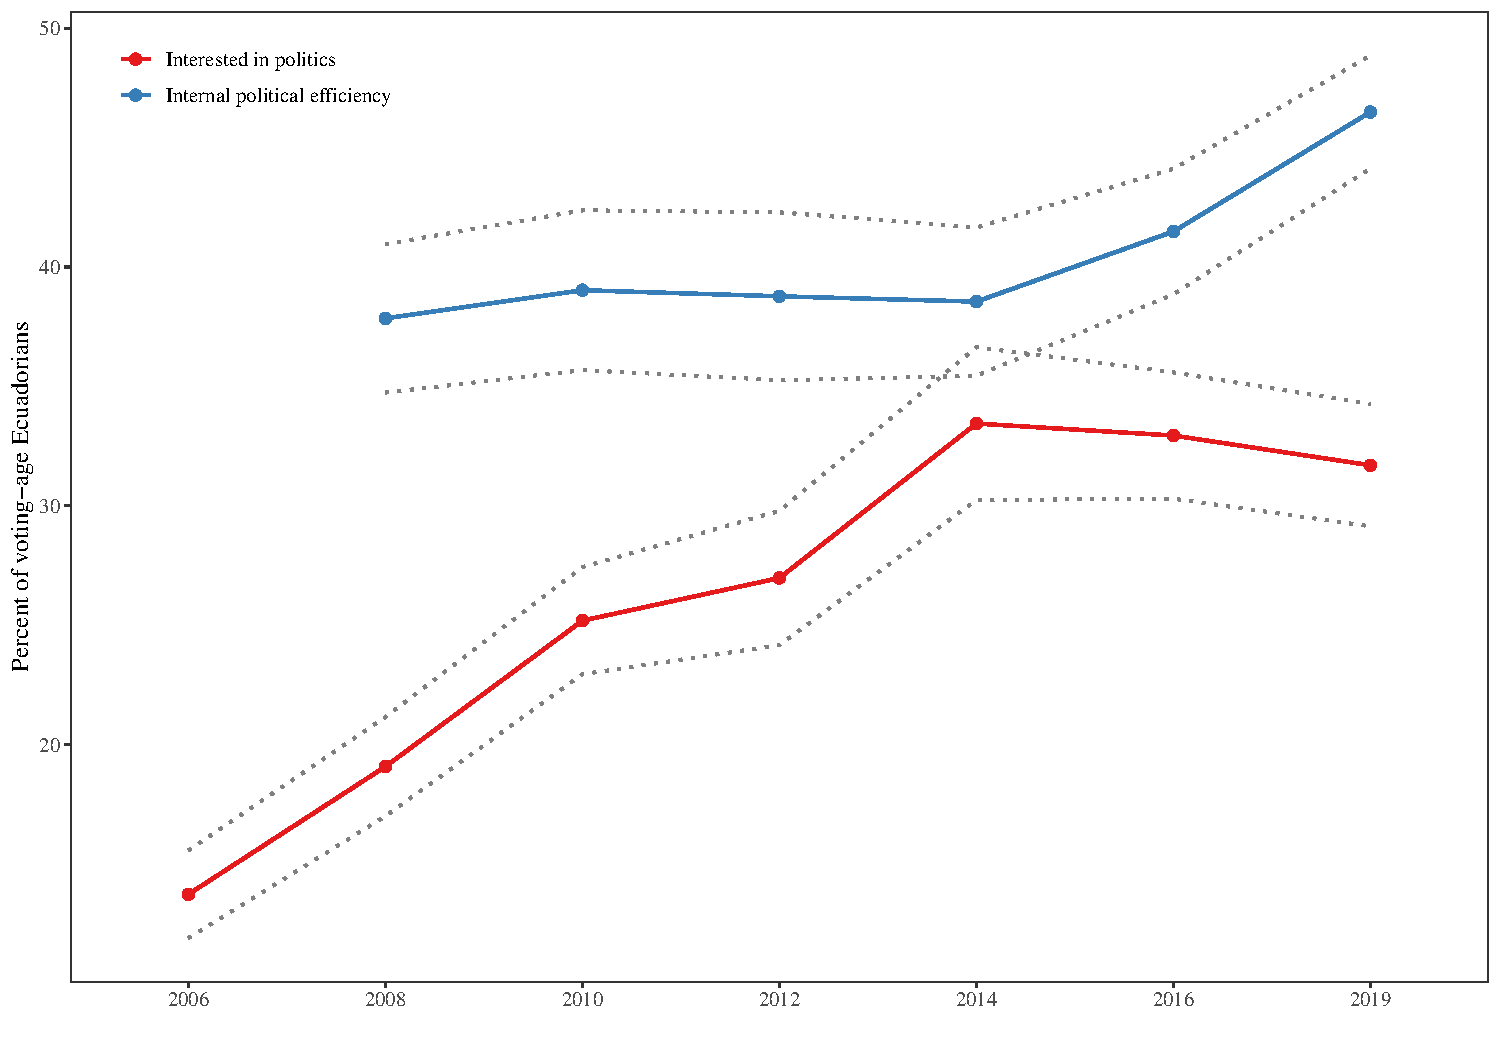
\includegraphics[width=\maxwidth]{figure/pol-int-graph-1} 

}


\end{knitrout}
\textbf{Note:} A time series of the internal political efficacy variable and the interest in politics variable. The internal political efficiency variable is dichotomized using the standard AB methodology as explained in \hyperref[app:first]{Appendix A}. Dotted lines represent the 95\% confidence intervals considering design effects. Data from the open-access AB databases. Figure prepared by the author.
\end{minipage}
}
\end{figure}

Figure \ref{fig:intpol} shows the percent who are interested in politics and also the percent who understand the country's politics. The gap between these two variables has increased from 2014 from 2016, and have a total historic correlation of 0.1938071. While they may appear to ask similar things, the two questions may imply different attitudes to politics: the political efficacy question simply asks if citizens are aware of politics and the second one asks if they're interested to enter the political scenario. It might be possible that, when separating these two questions, attitudes of apathy or pragmatism to the political society (understanding politics) are separated from an \enquote{idealist} attitude towards it of those who would like to enter politics.
\end{document}
